% subseccion 4.6
\subsection{Etapa 6: Resultados}
Este apartado presenta los resultados obtenidos a través de la ejecución del protocolo de búsqueda de la SMS. Inicialmente, se ofrece una descripción general de los datos correspondientes a los estudios primarios seleccionados SPS.

Esta descripción abarca aspectos como el origen de los estudios, el año de publicación, la estrategia de búsqueda utilizada para su localización, los índices de calidad, la relación con las preguntas de investigación (RQs) y sus respectivos temas, y las palabras clave. Por último, se presenta una descripción de una nube de palabras generada a partir de las palabras clave de los SPS.

Es importante recordar que la asociación entre los SPS y los temas se estableció mediante la clasificación detallada en la Sección \ref{subsec:clasificacion-de-estudios}. De manera inherente, las RQs también se asociaron, dado que los temas tienen una estructura específica dentro de ellas.

Asimismo, se identificó la asociación entre las principales palabras clave de la SMS con los títulos de las secciones, los resúmenes y las palabras clave en todos los SPS.

%sub-subseccion 4.6.1
\subsubsection{Descripción General de los SPSs (Estudios Primarios Seleccionados)}
El proceso de busqueda y filtrado de estudios resultó en la identificación de 114 SPSs como se muestra en la Tabla \ref{table:selected_primary_studies}.

\begin{figure}[htbp]
	\centering
	\vspace{10pt}
	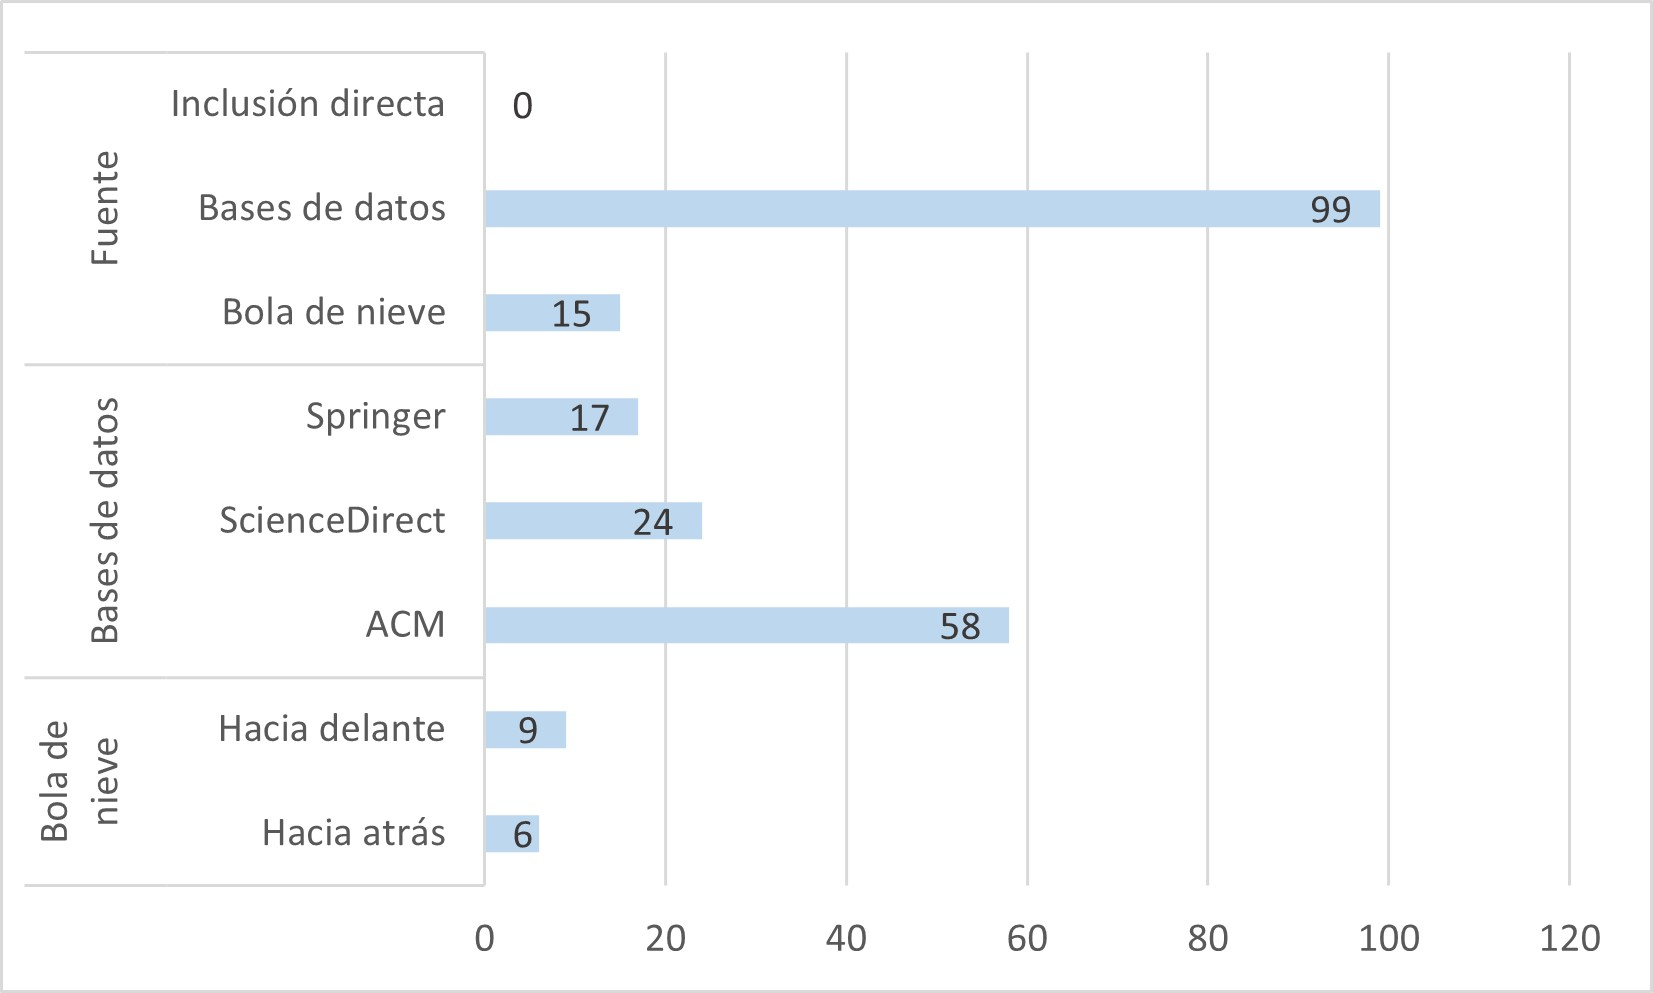
\includegraphics[scale=0.7]{resources/figures/SPSsByProcedence.jpg}
	\vspace{6pt}
	\caption{SPSs por procedencia y estrategia de búsqueda.}
	\label{fig:SPSsByProcedence}
\end{figure}

Estos SPSs vienen de bases de datos digitales, que identificamos en el SMS a través de diferentes estrategias. La Figura \ref{fig:SPSsByProcedence} muestra el numero de estudios identificados a través de varias fuentes y los detalles de las estrategias de busqueda en bases de datos y bola de nieve. Independientemente de la fuente, 86.84\% de los SPSs fueron encontrados a través de la estategia de búsqueda en bases de datos, mientras que el 13.16\% restante se identificó mediante la estrategia de bola de nieve.

Sin importar la estrategia de búsqueda en bases de datos, la Figura \ref{fig:SPSsByProcedence} muestra que de los 99 estudios encontrados a través de la estrategia de búsqueda en bases de datos, el 50.87\% fueron encontrados en la base de datos ACM, el 21.05\% en la base de datos ScienceDirect, y el 14.91\% en la base de datos Springer. Observando los 15 SPSs identificados por la estrategia de bola de nieve, el 40.00\% fueron encontrados mirando hacia atrás y el 60.00\% mirando hacia adelante.

\begin{figure}[htbp]
	\centering
	\vspace{10pt}
	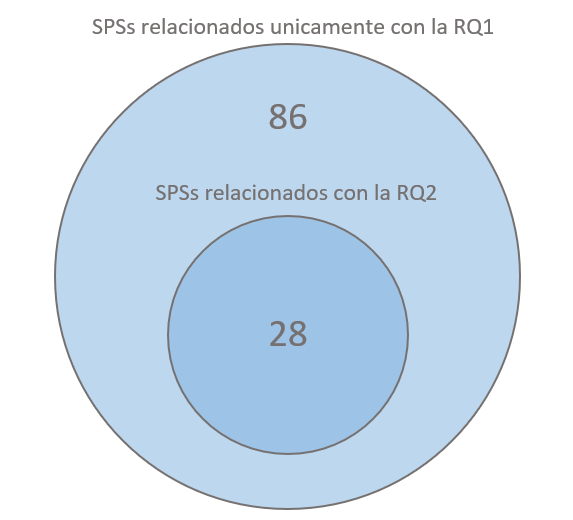
\includegraphics[scale=0.7]{resources/figures/Venn.png}
	\vspace{6pt}
	\caption{Relación de SPSs con las preguntas de investigación.}
	\label{fig:SPSsByRQs}
\end{figure}

Considerando las relaciones de los SPSs con las RQs, la Figura \ref{fig:SPSsByRQs} muestra que el 100.00\% de los SPSs están relacionados con la RQ1, Luego el 24.56\% de los SPSs están relacionados con ambas RQs simultaneamente. Por lo que el restante 75.44\% de los SPSs están relacionados unicamente con la RQ1. Mostrando así que no hay ningún SPS que esté relacionado exclusivamente con la RQ2.

\begin{figure}[htbp]
	\centering
	\vspace{10pt}
	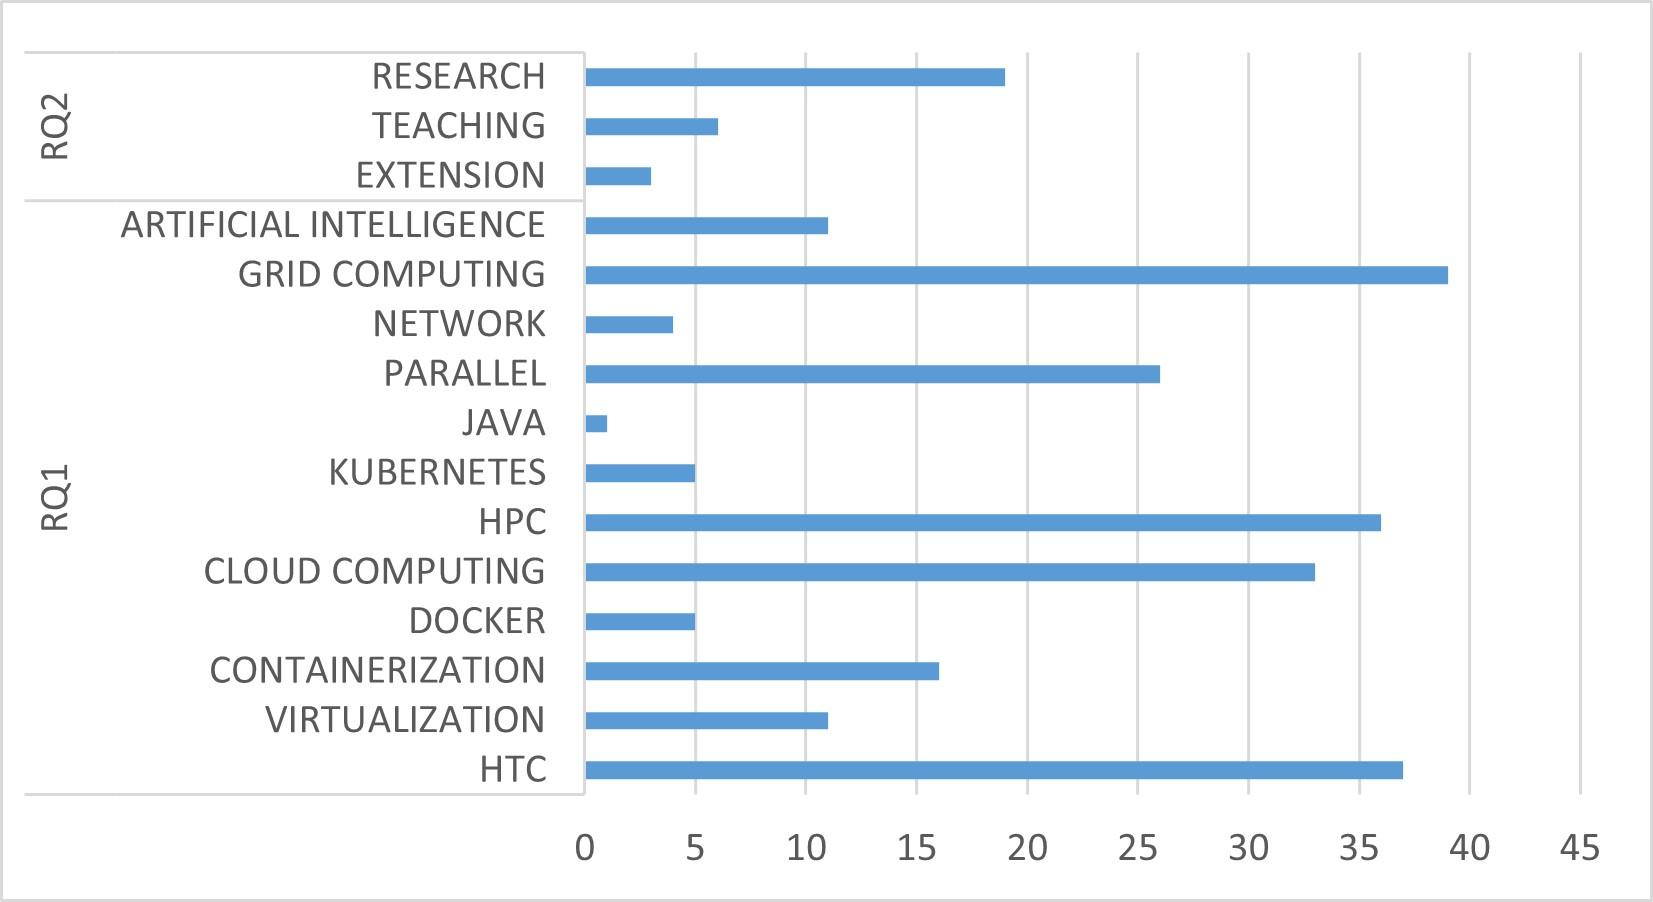
\includegraphics[scale=0.7]{resources/figures/SPSsByTopic.jpg}
	\vspace{6pt}
	\caption{Relación de SPSs con los tópicos de investigación.}
	\label{fig:SPSsByTopics}
\end{figure}

La Figura \ref{fig:SPSsByTopics} muestra los tópicos definidos en la etapa de planeación por cada pregunta de investigación y la cantidad de SPSs relacionados con cada topico de forma inclusiva. Es esencial tener en cuenta que un SPS puede estar relacionado con varios topicos simultaneamente. En este sentido, la Figura \ref{fig:SPSsByTopics} muestra los 14 topicos relacionados con la RQ1, de los que el topico ``Grid Computing'' es el más frecuente con 34.21\%. En contraste, los topicos con la menor frecuencia son ``Java'' y ``Checkpointing'' con 0.87\% ambos. Por otro lado, la Figura \ref{fig:SPSsByTopics} tambien muestra los 3 topicos relacionados con la RQ2, donde el topico ``Research'' es el más frecuente con 16.67\%, mientras que el topico con la menor frecuencia es ``Extension'' con 2.63\%.

\begin{figure}[htbp]
	\centering
	\vspace{10pt}
	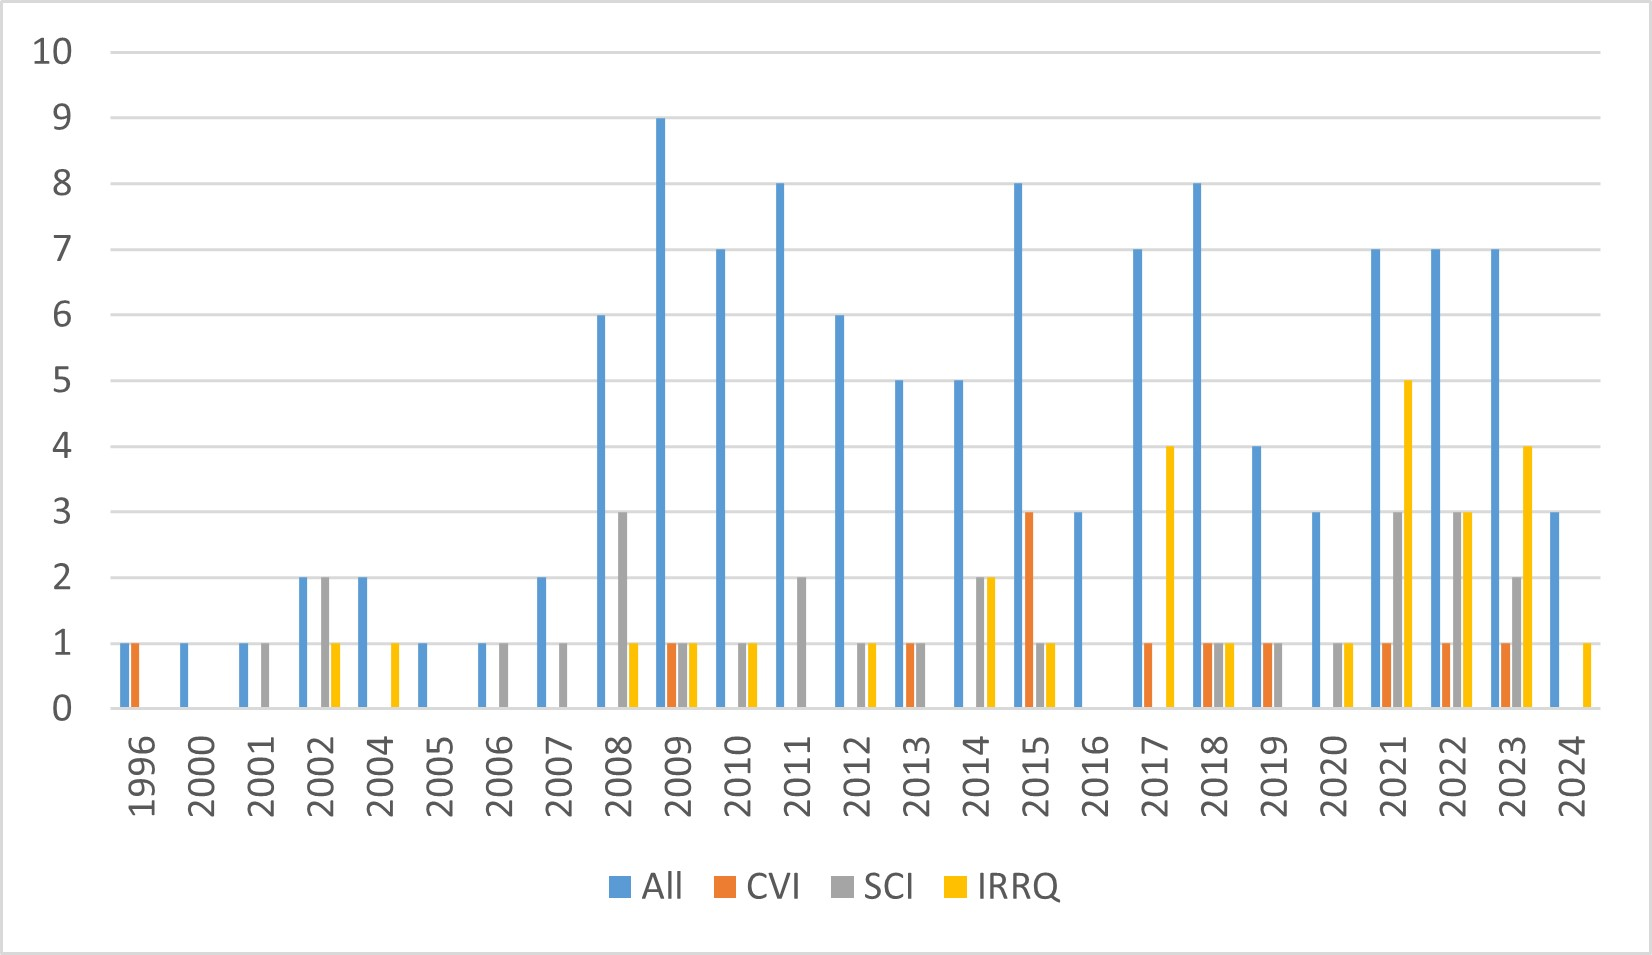
\includegraphics[scale=0.7]{resources/figures/SPSsBYearsAndIndexes.jpg}
	\vspace{6pt}
	\caption{Relación de SPSs con los años de publicación e índices de calidad.}
	\label{fig:SPSsByYearsAndIndexes}
\end{figure}

Se recalca que el periodo de busqueda va desde 1996 hasta 2024; en este sentido, la Figura \ref{fig:SPSsByYearsAndIndexes} muestra una baja cantidad de estudios publicados entre 1996 y 2007. Ver Figura \ref{fig:SPSsByYearsAndIndexes}. En contraste, en 2008 hubo un incremento respecto a 2007 con un total de 6 SPSs. El menor número de SPSs fue en el año 2009.

De acuerdo al indice SCI, este SMS presenta una distribución bastante regular a lo largo de todos los años, haciendo una excepción por los años entre 2006 y 2015, periodo en el que cada año se presenta al menos un SPS que cumpla con el indice SCI, lo cual, teniendo en cuenta la distribución y los intervalos parcialmente regulares en los que no aparece ningún SPS con este indice, se considera una anormalidad. Con respecto al indice CVI, el SMS muestra regularidad en la cantidad de SMSs por año, principalmente del 2017 hacia delante, excepto por el periodo entre 2000 y 2008, en el que no se encuentra ningún SPS que cumpla con el indice CVI. Considerando el indice IRRQ, el año 2021 registró la mayor cantidad de estudios que cumplieran con este criterio con un total de 5.Además, se evidencia una tendencia bastante regular en la cantidad de SPSs que cumplen con este indice a lo largo de los años.

\begin{figure}[htbp]
	\centering
	\vspace{10pt}
	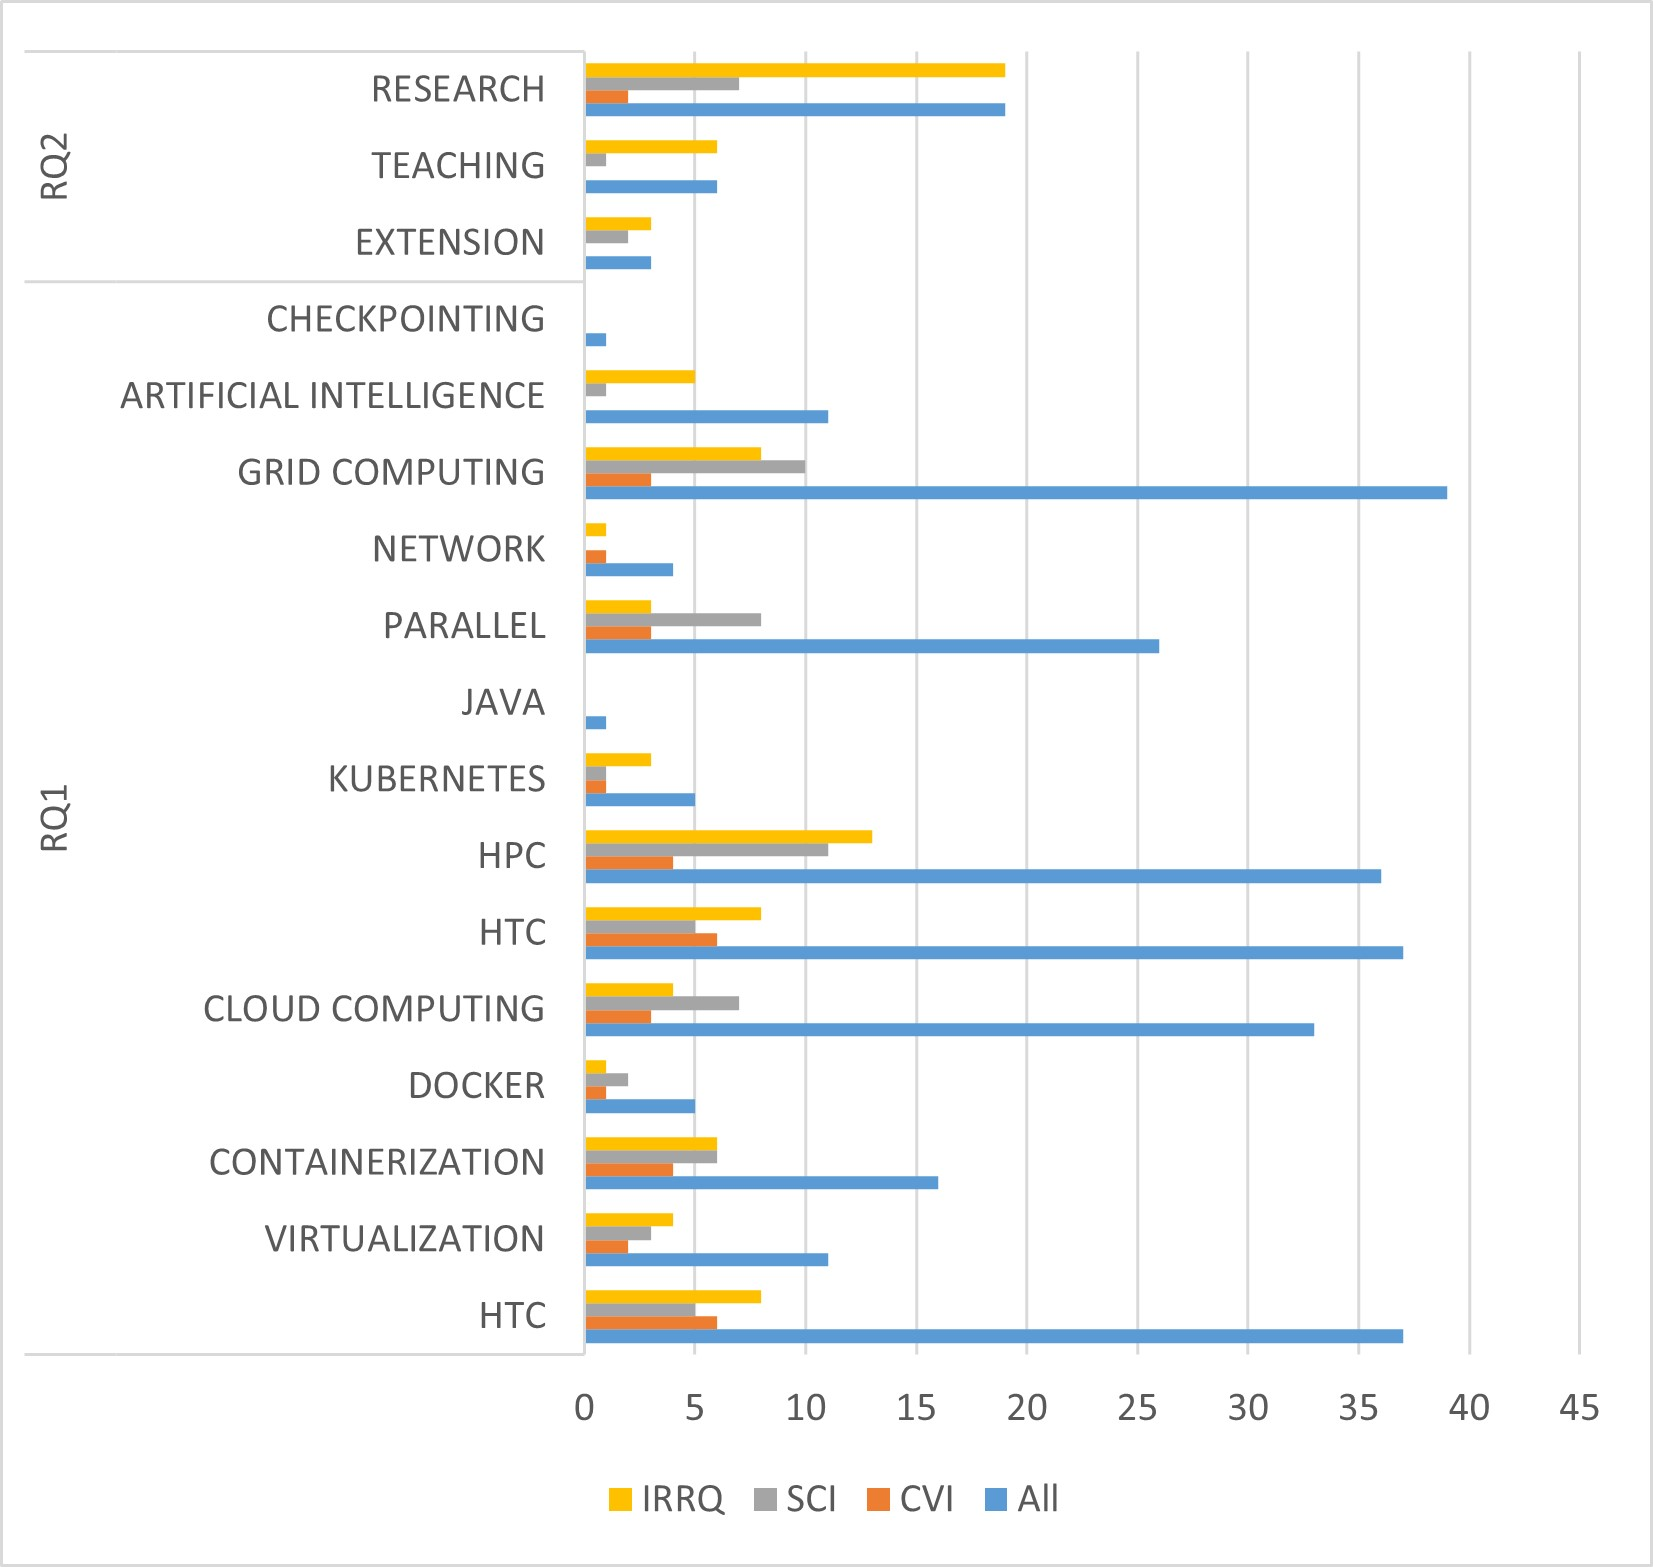
\includegraphics[scale=0.7]{resources/figures/IndexesByTopicAndRQs.jpg}
	\vspace{6pt}
	\caption{Índices de calidad por tópico y preguntas de investigación.}
	\label{fig:IndexesByTopicAndRQs}
\end{figure}

La Figura \ref{fig:IndexesByTopicAndRQs} muestra la cantidad de SPSs clasificados por pregunta de investigación e incluyendo sus respectivos topicos, adicionalmente se consideran los indices de calidad.

En este sentido, este estudio indica que para la RQ1, los topicos ``Java'' y ``Checkpointing'' registran la menor cantidad con 1 SPS, equivalente al 0.87\% de los 114 SPSs. En contraste, el topico ``Grid Computing'' es el más frecuente con 39 SPSs, equivalente al 34.21\% de los 114 SPSs. Por otro lado, para la RQ2, El topico más frecuente es ``Research'', con 19 SPSs equivalentes al 16.66\% de los 114 SPSs. En contraste, el topico ``Extension'' es el menos frecuente con 3 SPSs, equivalente al 2.63\% de los 114 SPSs.

Respecto a los indices CVI, SCI y IRRQ, identificamos los topicos ``Java'', ``Checkpointing'' y ``Extension'' como las categorias que más estudios contienen.

\begin{figure}[htbp]
	\centering
	\vspace{10pt}
	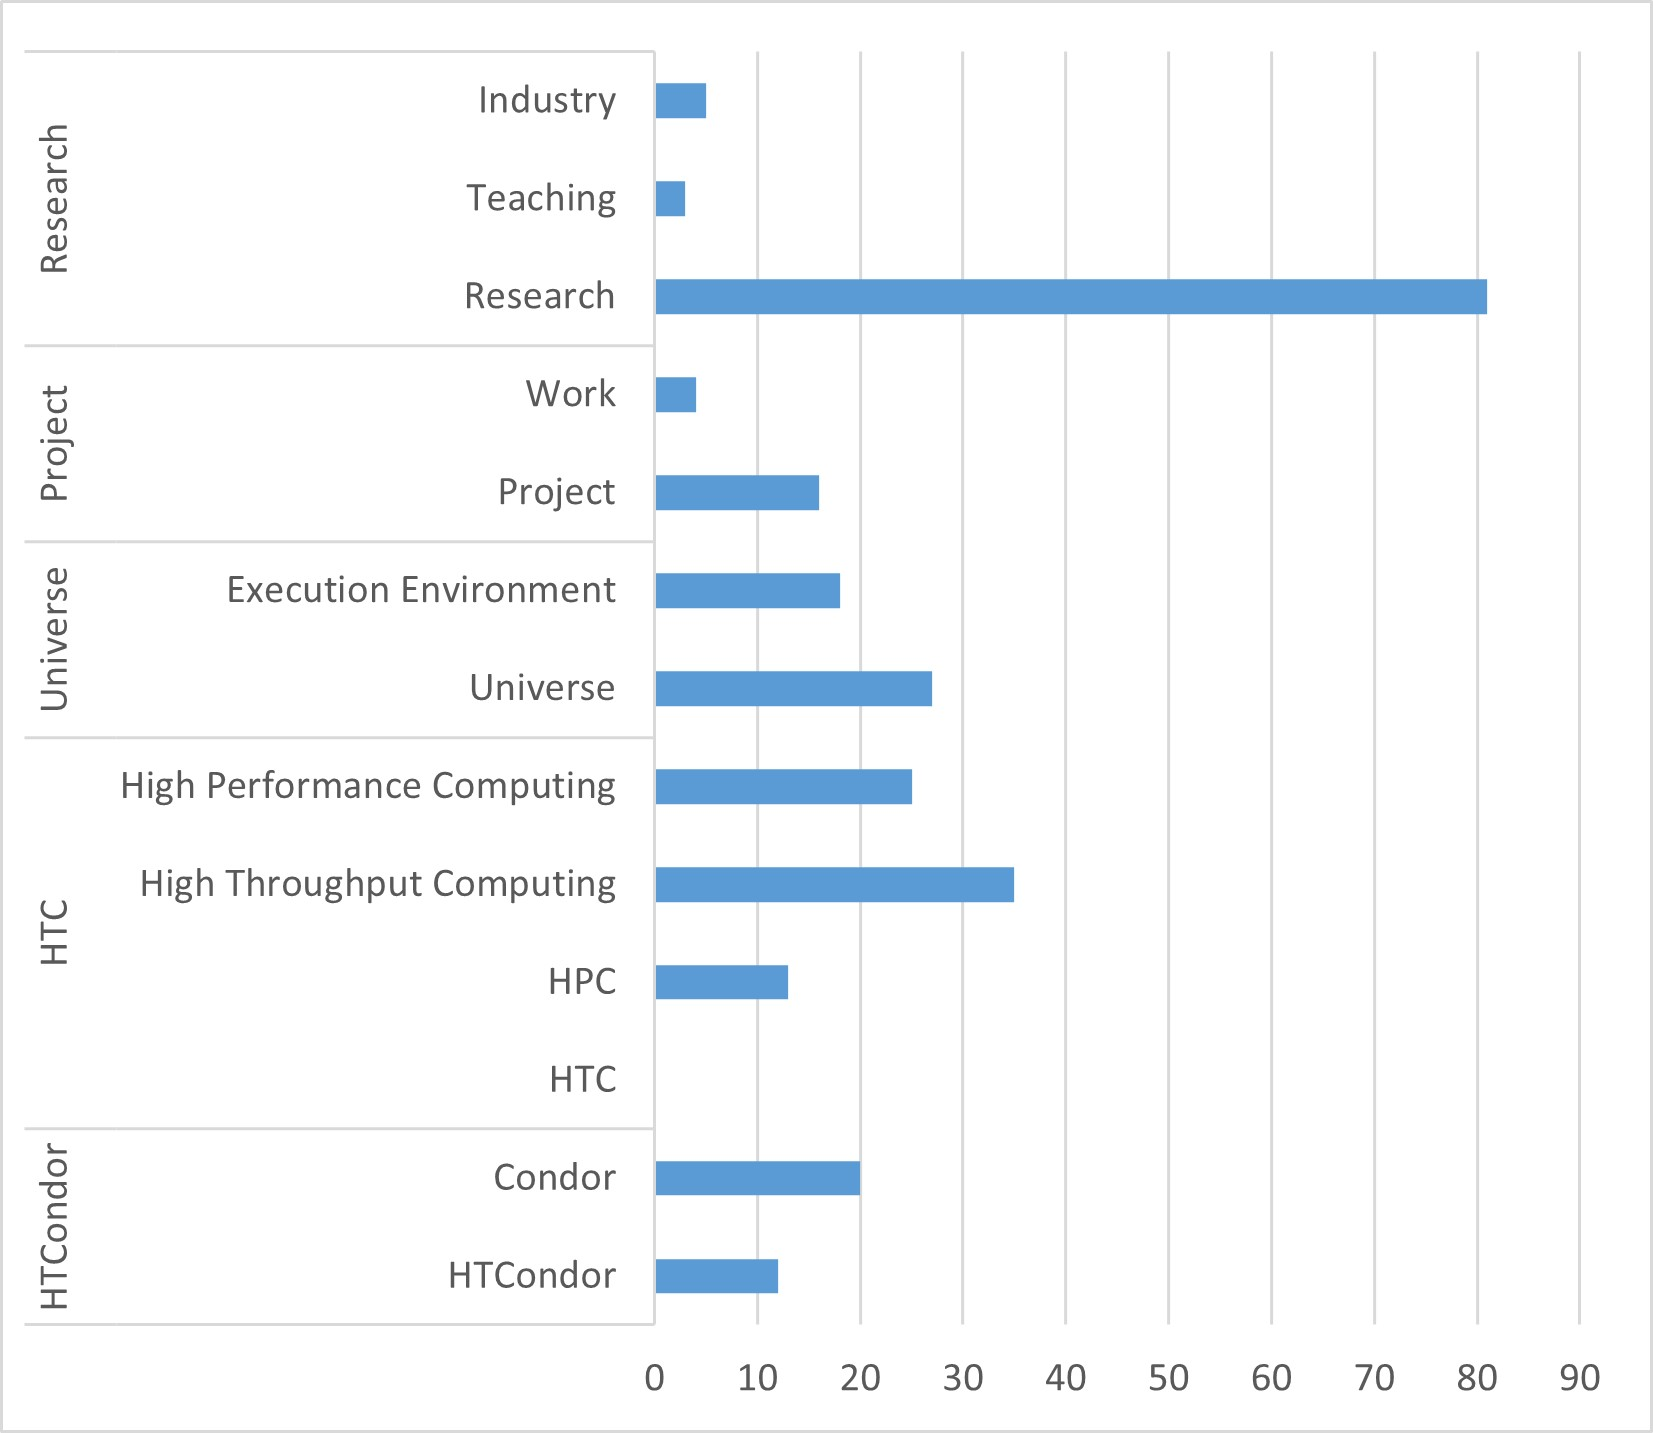
\includegraphics[scale=0.7]{resources/figures/SPSsByKeywords.jpg}
	\vspace{6pt}
	\caption{SPSs por palabras clave.}
	\label{fig:SPSsByKeywords}
\end{figure}

La Figura \ref{fig:SPSsByKeywords} muestra un analisis cruzado entre los SPSs, palabras clave y sinonimos. El sinonimo ``Work'' permitió la identificación de 81 SPSs. Respecto a la palabra clave ``Research'' permitió la identificación de 35 SPSs. Por otro lado la palabra clave ``Universe'' tiene la menor contribución, resultando en la identificación de ningún SPS.

%sub-subseccion 4.6.2
\subsubsection{Visualización de Nube de Palabras}

\begin{figure}[htbp]
	\centering
	\vspace{10pt}
	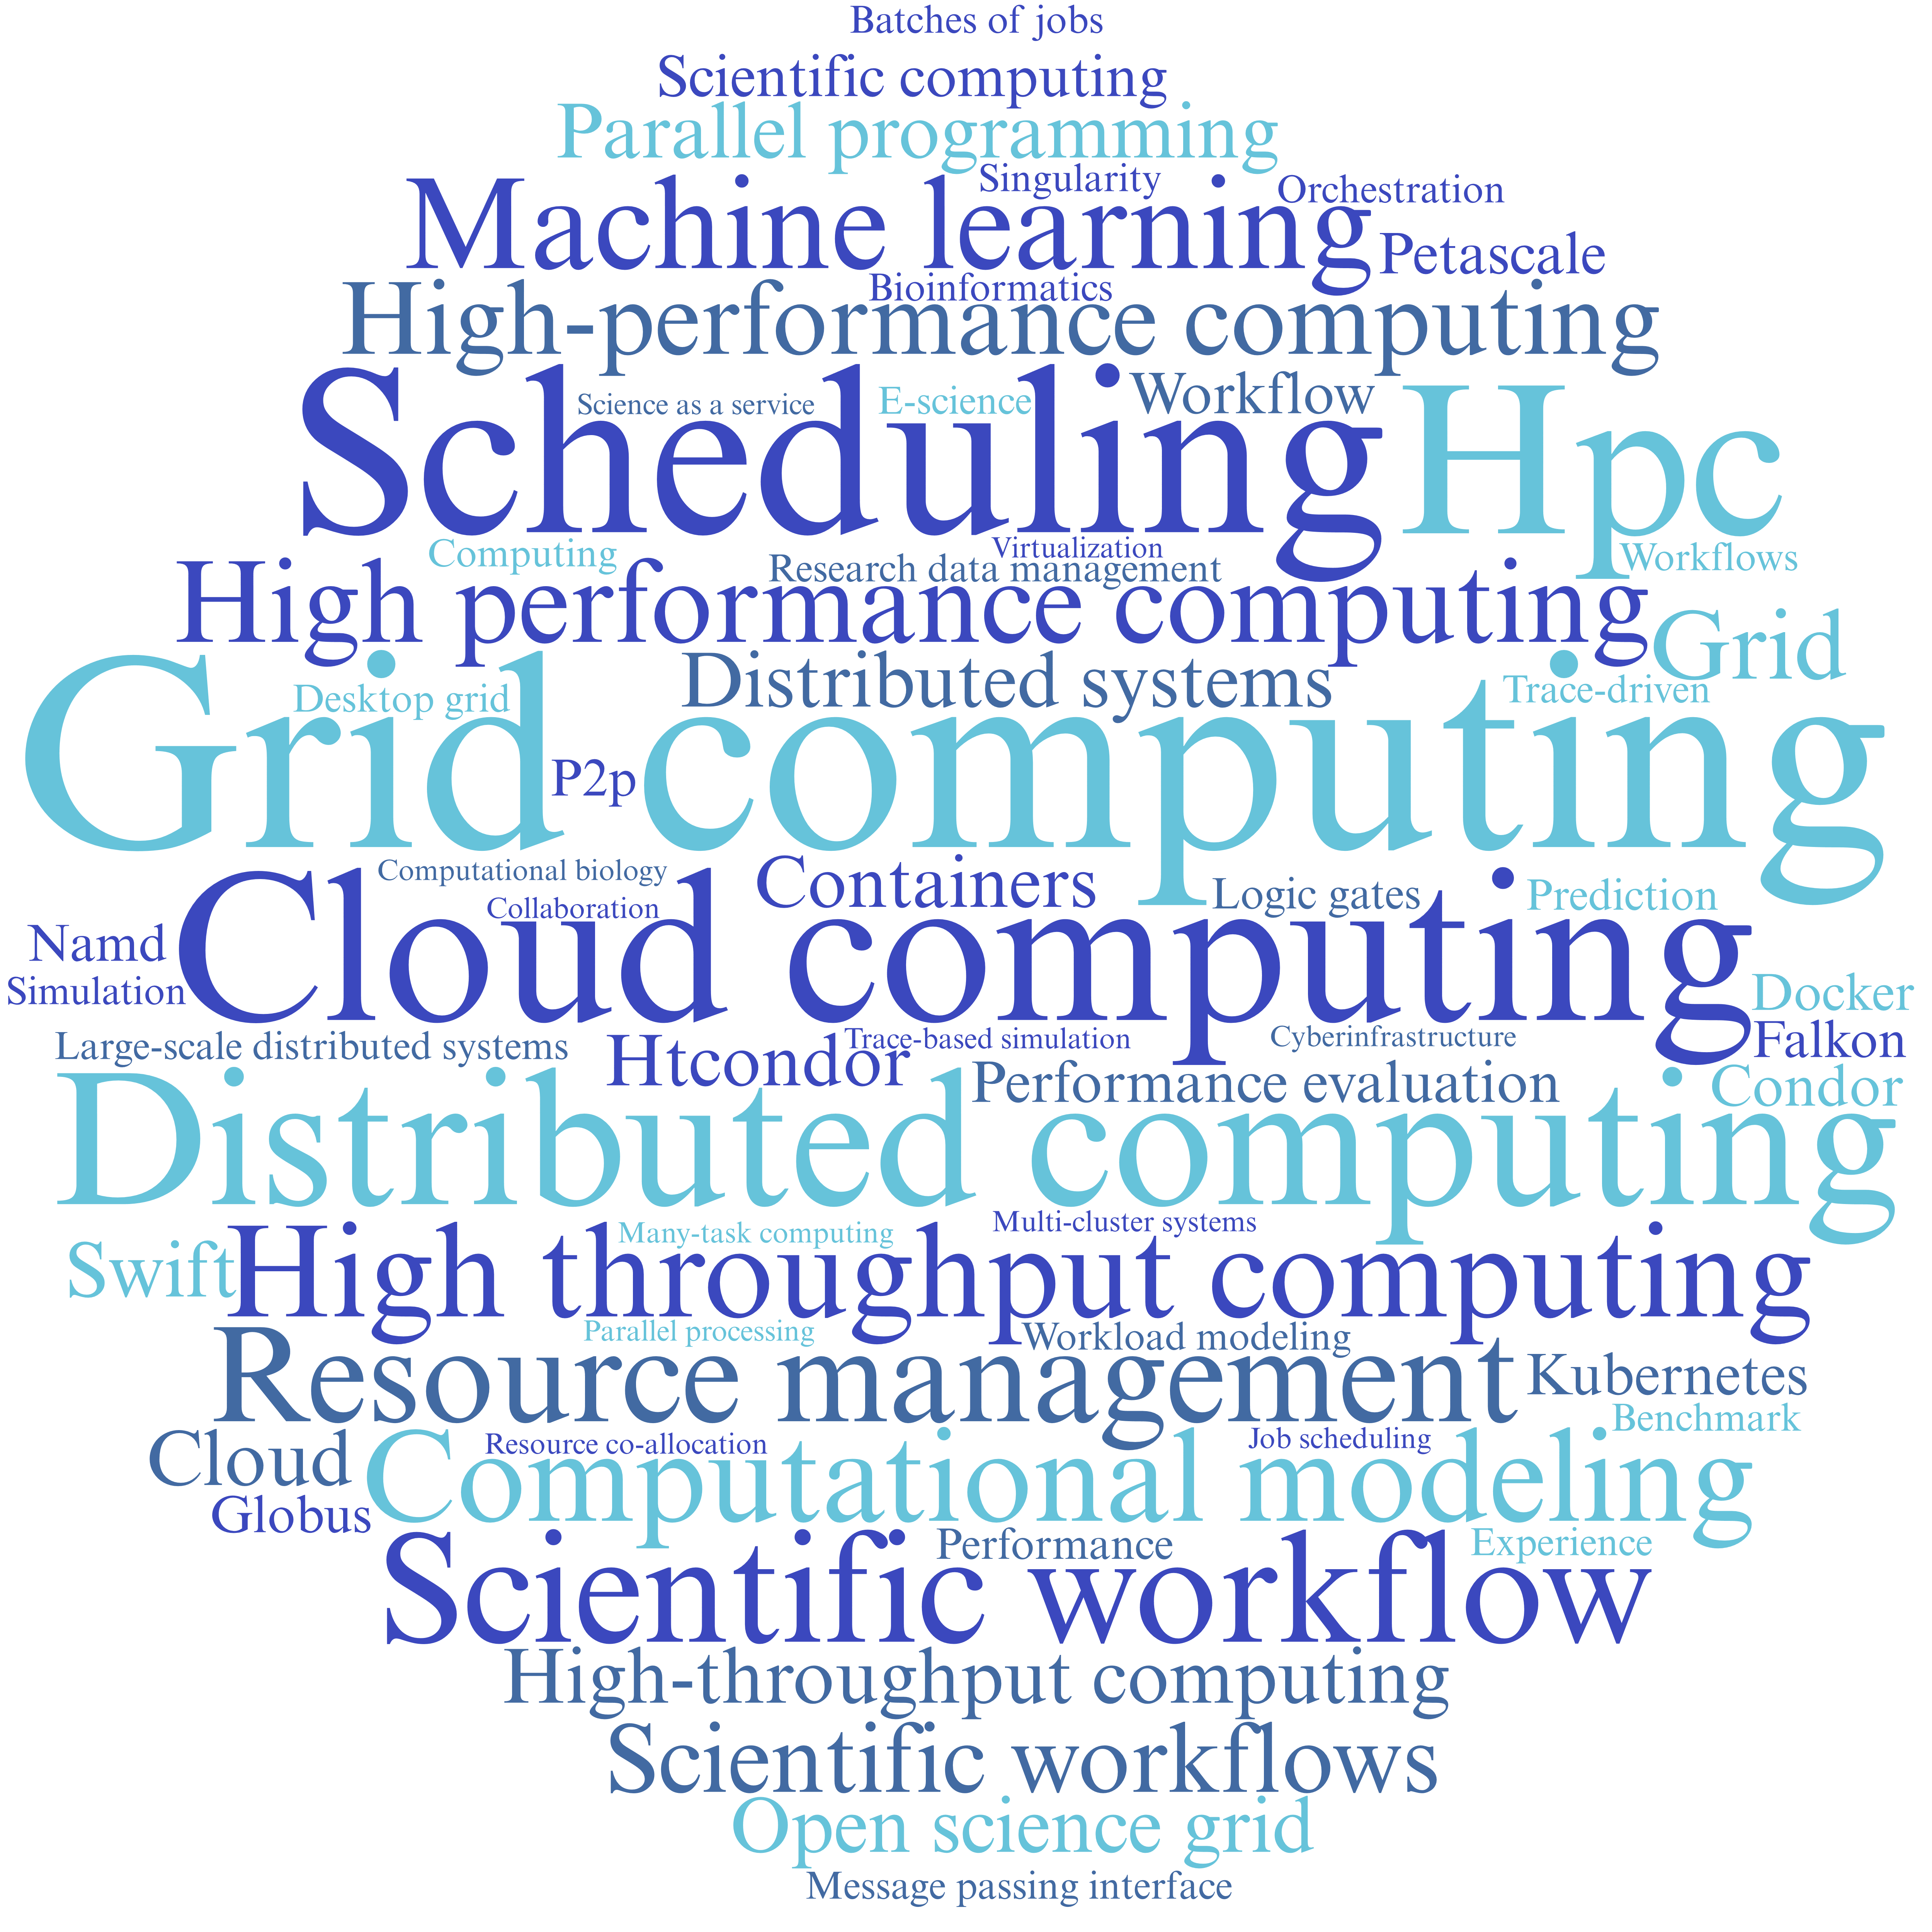
\includegraphics[scale=0.05]{resources/figures/wordcloud.png}
	\vspace{6pt}
	\caption{Nube de palabras de los palabras clave.}
	\label{fig:WordCloud}
\end{figure}

Otro resultado obtenido de los 114 SPSs del SMS, es la construcción de una nube de palabras. Con este tipo de grafico, se busca identificar las palabras y conceptos más frecuentes y que tienen la mayor importancia. La Figura \ref{fig:WordCloud} muestra la nube de palabras generada con la herramienta NubeDePalabras.es, cuya construcción se realizó a partir de las palabras clave de los SPSs.

Dentro de las palabras claves más frecuentes, se destacan ``Cloud computing'', ``Grid computing'' y ``Distributed computing'', con una contribución del 18.59\% en conjunto a la nube de palabras. El segundo nivel de relevancia en terminos de nube de palabras corresponden a ``HPC'', ``High Throughput Computing'' y ``Scheduling'', con una contribución del 11.98\%. Finalmente, tenemos un tercer nivel que incluye ``Resource Management'', ``High Performance Computing'' y ``Scientific workflow'', con una contribución del 7.85\%.

Cabe recalcar que los calculos se hicieron con base en las palabras tomadas para la nube, en este caso se excluyeron todas las palabras con solo una aparición en la nube de palabras, por lo que se uncluyeron todas las palabras con dos apariciones o más. Todo esto con el fin de extraer la información más relevante y no contaminar al lector con información no tan relevante. Luego, los porcentajes que se extrajeron fueron tomados de la cantidad de apariciones de las palabras con dos apariciones o más.
